\documentclass[a4paper, oneside]{book}
\usepackage[italian]{babel}
\usepackage[utf8]{inputenc}
\usepackage[a4paper,top=2.5cm,bottom=2.5cm,left=2cm,right=2cm]{geometry}
\usepackage{amssymb}
\usepackage{amsthm}
\usepackage{graphics}
\usepackage{amsfonts}
\usepackage{amsmath}
\usepackage{amstext}
\usepackage{engrec}
\usepackage{rotating}
\usepackage[safe,extra]{tipa}
\usepackage{multirow}
\usepackage{hyperref}
\usepackage{enumerate}
\usepackage{braket}
\usepackage{marginnote}
\usepackage{pgfplots}
\usepackage{cancel}
\usepackage{polynom}
\usepackage{booktabs}
\usepackage{enumitem}
\usepackage{algorithm}
\usepackage{algpseudocode}
\usepackage{framed}
\usepackage{pdfpages}
\usepackage{pgfplots}
\usepackage{fancyhdr}
\usepackage{caption}
\usepackage{subcaption}
\usepackage{setspace}
\usepackage{hyperref}
\pagestyle{fancy}
\fancyhead[L,RO]{\slshape \rightmark}
\fancyfoot[C]{\thepage}

\title{Visual Information Processing and Management}
\author{Tommaso Ferrario (\href{https://github.com/TommasoFerrario18}{@TommasoFerrario18}) \\\\
Telemaco Terzi (\href{https://github.com/Tezze2001}{@Tezze2001})}
\date{Ottobre 2024}

\pgfplotsset{compat=1.13}

\begin{document}

\maketitle
\newtheorem{teorema}{Teorema}
\newtheorem{dimostrazione}{Dimostrazione}
\newtheorem{definizione}{Definizione}
\newtheorem{esempio}{Esempio}
\newtheorem{osservazione}{Osservazione}
\newtheorem{nota}{Nota}
\newtheorem{corollario}{Corollario}
\tableofcontents
\renewcommand{\chaptermark}[1]{
    \markboth{\chaptername
        \ \thechapter.\ #1}{}}
\renewcommand{\sectionmark}[1]{\markright{\thesection.\ #1}}

\chapter{Colori}
I colori possono essere descritti in termini:
\begin{itemize}
    \item \textbf{fisici}: attraverso la distribuzione spettrale di energia,
          fattore di riflessione, gloss\dots
    \item \textbf{sensoristica}: stimolazione dei fotorecettori dell'occhio attraverso
          le radiazioni elettromagnetiche.
    \item \textbf{psicologica}: impressione soggettiva del colore condizionata
          dalla situazione dell'osservatore e i materiali degli oggetti.
\end{itemize}

Il colore è frutto della combinazioni di diverse componenti:
\begin{itemize}
    \item distribuzione spettrale di energia illuminante: specifica quale colore
          viene emesso dalla luce.
    \item distribuzione spettrale di riflettanza: specifica quali colori vengono
          assorbiti dall'oggetto e quali colori vengono riflessi dall'oggetto.
    \item quantità di fotoni assorbiti dall'occhio umano.
    \item sensibilità dei coni che assorbono i singoli colori della luce.
\end{itemize}

L'occhio umano è composto da:
\begin{itemize}
    \item iride: si occupa di far passare la luce nell'occhio
    \item cristallino: si occupa di regolare il fuoco
    \item retina: si occupa di assorbire il colore
\end{itemize}

Sulla retina sono presenti:
\begin{itemize}
    \item rods: si occupano della vista scotopica utile per vedere i movimenti (funzionano con scarsa luce)
    \item cones: si occupano di recepire il colore (funzionano con una buona luce)
\end{itemize}

I coni degli sono sensibili alle lunghezze d'onda dei colori blu, rosso e verde.
Le curve rosse e verdi sono più sovrapposte perché in questo modo si possono
riconoscere più sfumature composte da questi colori.

Dal momento che gli esseri umani hanno una percezione del colore a tre dimensioni
questo viene detto \textbf{tristimulus color} e i singoli componenti vengono chiamati:
\begin{itemize}
    \item \textbf{short}: percepisce le onde corte e quindi il blu:
          \begin{equation*}
              S = \int_{\lambda} \phi(\lambda) S(\lambda)d\lambda
          \end{equation*}
    \item \textbf{medium}: percepisce le onde medie e quindi il verde
          \begin{equation*}
              M = \int_{\lambda} \phi(\lambda) M(\lambda)d\lambda
          \end{equation*}
    \item \textbf{long}: percepisce le onde lunghe e quindi il rosso
          \begin{equation*}
              L = \int_{\lambda} \phi(\lambda) L(\lambda)d\lambda
          \end{equation*}
\end{itemize}

Le formule specificate precedentemente specificano la quantità massima di fotoni
percepibili dai coni di un essere umano.

Quindi per assorbire il colore, data una distribuzione spettrale di energia e
la sensibilità dei tre coni, si calcolano $3$ distribuzioni colore ottenute dall'intersezione
tra l'area di ciascun cono e quella della distribuzione del colore. Il colore è
data dalla tripla $R,G,B$  ottenute dall'integrale delle $3$ distribuzioni definite
precedentemente.

\begin{nota}
    I coni effettuano una discretizzazione del colore in $3$ canali
\end{nota}

In aggiunta tutti gli spettri che stimolano la stessa risposta dei coni sono
indistinguibili e in caso si chiamano \textbf{metameric matches}. In realtà
abbiamo 3 diverse metameric match:
\begin{itemize}
    \item \textbf{Color metamerism}: due spettri sono identici sotto lo stesso
          osservatore e la stessa luce.
    \item \textbf{Illumination metamerism}: due spettri sono identici sotto la
          stessa illuminazione.
    \item \textbf{Observer metamerism}: due spettri sono identici sotto lo stesso
          osservatore.
\end{itemize}
\section{Colorimetry}
\begin{definizione}[Colorimetry]
    La \textbf{colorimetry} è la branca della scienza del colore che si occupa
    di specificare numericamente il colore in modo che:
    \begin{itemize}
        \item se il colore viene visto da un osservatore normale, sotto le stesse
              condizioni deve essere uguale.
        \item colori uguali devono avere la stessa rappresentazione.
        \item le codifiche devono essere associate a funzioni fisiche.
    \end{itemize}
\end{definizione}

L'obiettivo è di mappare tutti i colori visibili in codifiche standard basate sulla
combinazione di colori primari.

\begin{definizione}[Grassman's law]
    La legge di \textbf{Grassman's law} è la legge che specifica che un colore può
    essere ottenuto da una combinazione lineare di una serie di colori primari.
\end{definizione}

\subsection{CIE RGB}
Una delle prime codifiche dei colori è la \textbf{CIE RGB} la quale si basa su
uno studio in cui i partecipanti correggere dei sensori modificando la quantità
dei colori primari per ottenere il colore target.

Risulta importante notare che questo standard ammette anche contributi negativi,
ovvero si ha la possibilità di sottrarre il contributo di un particolare colore.
Questo viene fatto aggiungendo al colore target la parte che viene sottratta.
\begin{nota}
    La codifica appena presentata rispetta la legge di Grassman.
\end{nota}
\subsection{CIE XYZ}
Il problema della codifica \textit{CIE RGB} è che si hanno contributi negativi,
di conseguenza, si è passati a un nuovo standard \textbf{CIE XYZ}. Sfruttando il
fatto che lo spazio di color matching è lineare, si è passati alla codifica \textbf{CIE XYZ}
inserendo i seguenti vincoli:
\begin{itemize}
    \item Il canale Y rappresenta la luminanza.
    \item Nelle curve che rappresentano i colori non ci sono valori negativi.
    \item Il colore bianco è ottenuto come: $1/3, 1/3, 1/3$
\end{itemize}
Il problema di questa codifica è che i primari non sono colori che esistono nella
realtà perciò non sono visibili. In aggiunta, la codifica rispetta anche il terzo
principio della \textbf{colorimetry}, ovvero le codifiche dipendono da una
rappresentazione fisica infatti:
\begin{equation*}
    \begin{array}{c}
        X = \int_{380}^{780} l(\lambda) \overline{x}(\lambda)d \lambda \\\\
        Y = \int_{380}^{780} l(\lambda) \overline{y}(\lambda)d \lambda \\\\
        Z = \int_{380}^{780} l(\lambda) \overline{z}(\lambda)d \lambda \\\\
    \end{array}
\end{equation*}

Dove $380-780$ sono  le frequenze visibili all'occhio umano e $\overline{x},
    \overline{y},\overline{z}$ sono i colori primari.

I colori dello spazio XYZ sono sul piano di intersezione tra i tre colori primari
e nel piano non tutti i punti sono colori reali.

Visto che i colori sono rappresentanti su un piano è stata definita la codifica
\textbf{CIE xyY} che specifica il colore usando una componente per la
\textbf{luminanza} e due componenti per la \textbf{cromaticità}.

Lo spazio colore xyY ha i colori puri sulla frontiera e il bianco è nella parte
centrale.

\begin{definizione}[Gamma cromatica]
    La \textbf{gamma cromatica} è l'insieme di tutti i colori rappresentabili
    dalla combinazione lineare di un insieme di colori primari.
\end{definizione}

Nel diagramma di cromaticità xyY, specificando un numero finito di colori primari
si può formare una forma convessa la quale contiene tutti i colori rappresentabili
da quelli primari specificati. Ciò risulta utile trovare un modo per comparare i
colori, questo potrebbe essere risolto attraverso una misura di distanza, il
problema è che sullo spazio XYZ o xyY le distanze normali non corrispondono alla
similarità del colore percepita.

Una dimostrazione di ciò sono gli \textbf{ellissi MacAdam}, ovvero ellissi che
racchiudono colori che sono percepibili simili. Questi non sono uniformi su tutto
il piano quindi le normali distanze non funzionano.
\subsection{CIE-LAB}
Per risolvere questo problema si passa a allo spazio colore con colori opponenti,
ovvero la prima componente deve essere quella \textbf{acromatica} (lucentezza) (0/100),
\textbf{rosso-verde} (-100/100) e infine \textbf{giallo-blu} (-100/100). Nella
trasformazione del canale di lucentezza si hanno due casi in base al fatto se si
ha tanta luce o meno per modellare il fatto che, a luce soffusa, il contributo
al colore viene dato da coni e dai bastoncini.

Questo standard viene chiamato \textbf{CIE-LAB} e permette l'utilizzo della norma
euclidea per confrontare i colori. L'unico problema rimanente è trovare la threshold
sulla distanza per dire che due colori sono uguali, questo dipende interamente dal
dominio.

\textbf{CIE} ha elaborato degli standard per le sorgenti luminose e la loro
temperatura come $D65$ e $D50$.

Nell'ambito dei colori è utile avere degli strumenti che li misurano:
\begin{itemize}
    \item Spettro-radiometro: misura la distribuzione spettrale di energia.
    \item Colorimetro: misura i valori di tristimolo assumendo la luce D65 e D50
          come reference del bianco.
    \item Spettrofotometro: misura la curva di riflettanza dell'oggetto
\end{itemize}
Per ogni strumento dobbiamo abbiamo due caratteristiche:
\begin{itemize}
    \item \textbf{Precisione}: quante volte misurando lo stesso oggetto otteniamo
          la stessa misura
    \item \textbf{Accurato}: quanto si avvicina la misura al valore vero.
\end{itemize}

\section{Acquisizione dell'immagine e sensibilità}
L'immagine viene generata dalla combinazione della sorgente di illuminazione e
dalle rifrazioni degli oggetti nella scena. Quando dobbiamo acquisire un'immagine
in digitale dovremmo generare una matrice di pixel che rappresenta la luce nella
scena. Per creare l'immagine digitalizzata è necessario effettuare due passi:
\begin{itemize}
    \item \textbf{sampling}: discretizzazione dei pixel
    \item \textbf{quantizzazione}: discretizzazione dei colori
\end{itemize}

Definiremo in seguito la \textbf{risoluzione spaziale} ovvero la dimensione dei
singoli pixel o anche il numero di pixel un'unità di distanza ed è dipendente dal
sampling rate.

Definiremo la \textbf{risoluzione di intensità} ovvero il numero di bit usati per
la quantizzazione.

Le risoluzioni producono degli artefatti:
\begin{itemize}
    \item risoluzione spaziale troppo piccola produce contorni spigolosi
    \item risoluzione di intensità troppo bassa produce dei falsi contorni
\end{itemize}

La prima risoluzione è sensibile alle variazione della forma mentre la seconda è
sensibile alle variazioni dell'intensità.

\chapter{Operatori sulle immagini}
Per ogni pixel possiamo definire due tipologie di vicinato:
\begin{itemize}
    \item \textbf{vicinato di Von Neumann}: se il pixel è $x,y$ il vicinato è
          \begin{equation*}
              (x-1, y) \ (x, y-1) \ (x+1, y) \ (x, y+1)
          \end{equation*}
    \item \textbf{vicinato di Moore}: se il pixel è $x,y$ il vicinato è:
          \begin{equation*}
              (x-1, y) \ (x-1, y-1) \ (x, y-1) \ (x+1, y-1) \ (x+1, y) \ (x+1, y+1)
              \ (x, y+1) \ (x-1, y+1)
          \end{equation*}
\end{itemize}
Possiamo definire il \textbf{percorso digitale} tra due pixel come la sequenza di
pixel che separano i due di interesse. La \textbf{lunghezza del cammino} sarà il
numero di edge del percorso, ricorda che la scelta del vicinato fa variare i vari
cammini disponibili. Si definisce \textbf{cammino chiuso} come il percorso da un
pixel a se stesso.

Dato $S$ un insieme di pixel allora due pixel $p$, $q$ sono \textbf{connessi} in
$S$ se esiste un percorso in $S$ tra i due formato solo da pixel in $S$. L'insieme
dei pixel connessi in $S$ si chiama \textbf{componente connessa}, se esiste una
sola componente ed è connessa allora $S$ è chiamato \textbf{insieme connesso}.

Sia $R$ un sottoinsieme di pixel dell'immagine, $R$ è una \textbf{regione} dell'immagine
se è un insieme connesso. Date due regioni $R_1,R_2$, se sono \textbf{adiacenti}
allora la loro unione forma un insieme connesso altrimenti sono disconnessi.

\begin{nota}
    Le definizioni variano in base alla vicinanza.
\end{nota}

Date delle regioni disgiunte allora, ogni singola regione può essere chiamata
\textbf{foreground} mentre il complemento è il \textbf{background}. Definite le
regioni possiamo definire due bordi:
\begin{itemize}
    \item bordo interno sono i pixel del foreground adiacenti ai pixel del background
    \item bordo esterno sono i pixel del background adiacenti ai pixel del foreground
\end{itemize}

Possiamo definire diverse distanze tra i pixel:
\begin{itemize}
    \item \textbf{euclidea}:
          \begin{equation}
              D_e(p,q) = \sqrt{(x_p-x_q)^2+(y_p-y_q)^2}
          \end{equation}
    \item \textbf{city-block}:
          \begin{equation}
              D_4(p,q) = |x_p-x_q|+|y_p-y_q|
          \end{equation}
    \item \textbf{chessboard}:
          \begin{equation}
              D_8(p,q) = max(|x_p-x_q|,|y_p-y_q|)
          \end{equation}
\end{itemize}

Definiremo diverse tipologie di operazioni:
\begin{itemize}
    \item \textbf{Operazioni element-wise}: operazioni puntuali tra due matrici
    \item \textbf{Operazioni matriciali}: operazioni tra matrici
    \item \textbf{Operazioni lineari}: operatori $\mathcal{H}[f(x,y)] = g(x,y)$
          che soddisfano le seguenti proprietà:
          \begin{itemize}
              \item omogeneità: dominio uguale al codominio
              \item additività: $\mathcal{H}[\alpha f_1(x,y) + \beta f_2(x,y)] =\alpha  \mathcal{H}[f_1(x,y)] + \beta  \mathcal{H}[f_2(x,y)] $
          \end{itemize}
\end{itemize}

Si possono definire \textbf{operazioni aritmetiche} tra immagini ovvero $+, -, \cdot, \%$
che sono element-wise e applicabili su immagini delle stesse dimensioni.

\begin{nota}
    Se da una immagine rumorosa applichiamo una media della immagine con la stessa con
    diversi noise di media nulla allora riduciamo la varianza del noise sull'immagine.
\end{nota}
\begin{nota}
    Possiamo comparare le immagini mediante la loro differenza.
\end{nota}
\begin{nota}
    Possiamo correggere le ombre mediante le operazioni di prodotto e divisione.
\end{nota}

Ogni volta che applichiamo operazioni sulle immagini rischiamo di uscire dalla
quantizzazione utilizzata quindi dobbiamo sempre \textbf{clippare} e \textbf{scalare}.
Per farlo usiamo la seguente funzione:
\begin{equation}
    g_s(x,y) = K\frac{g(x,y) -g_{min}}{g_{max} g_{min}}
\end{equation}
dove $K$ è la massima intensità rappresentabile nella quantizzazione scelta e
$g_{min}, g_{max}$ sono rispettivamente la minima e la massima intensità riscontrata
nell'immagine.

Si possono definire le \textbf{operazioni insiemistiche} sulle immagini. Per
prima cosa bisogna definire le immagini secondo insiemi:
\begin{equation}
    A = \{ (x,y,z) \}
\end{equation}
dove $x,y$ sono le coordinate spaziali mentre $z$ è l'intensità, quindi le operazioni
si baseranno su questa definizione, per esempio:
\begin{equation}
    A^c=\{(x,y, K-z) |(x,y, K-z) \in A\}
\end{equation}
\begin{equation}
    A\cup B=\{max_z(a,b) |a \in A, b\in B\}
\end{equation}

Possiamo applicare anche \textbf{operazioni logiche} che si possono applicare solo
su immagini binarie, ovvero $\land, \lor, \lnot$.

Possiamo applicare anche \textbf{operazioni spaziali}, le quali si dividono in:
\begin{itemize}
    \item \textbf{single-pixel}: modificano i pixel individualmente mediante una
          trasformazione $T$ (funzione continua) dove $z$ è l'intensità iniziale
          del pixel e $s$ è quella trasformata:
          \begin{equation}
              s=T(z)
          \end{equation}
    \item \textbf{neighborhood}: operano sull'intensità basandosi sull'intensità
          dei pixel vicini (filtri)
    \item \textbf{geometric transformation}: non cambiano l'intensità ma trasformano
          le coordinate geometriche dei pixel attraverso \textbf{trasformazioni
              affini} dello spazio, quindi applicano traslazioni, scaling,
          rotazioni e shearing. Le trasformazioni affini preservano punti, linee
          e piani. Dal momento che le trasformazioni sono affini allora possiamo
          concatenare una serie di trasformazioni applicando un prodotto tra matrici.
          Dopo ciascuna trasformazione spaziale si applica sempre una interpolazione
          dell'intensità in modo da applicare un antialiasing, per fare questo
          passo si usano i seguenti metodi:
          \begin{itemize}
              \item nearest neighbor: si prende il pixel più vicino agli angoli e si usa
                    il suo colore.
              \item bilinear interpolation: servono $4$ vicini
              \item bicubic interpolation: servono $16$ vicini
          \end{itemize}
\end{itemize}

Spesso quando si devono risolvere dei task si passano le immagini ad uno
\textbf{spazio trasformato}, in generale significa che abbiamo una funzione
$r(x,y,u,v)$ chiamata \textbf{forward trasnformation kernel} che trasforma ciascun
pixel:
\begin{equation}
    T(u,v) = \sum_r \sum_c f(r,c) r(r,c,u,v)
\end{equation}
Per ogni trasformazione esiste sempre l'inversa per tornare a quella originaria
\begin{equation}
    f(r,c) = \sum_u \sum_v T(u,v) r^{-1}(r,c,u,v)
\end{equation}

Parleremo di forward trasnformation kernel \textbf{separabili} se:
\begin{equation}
    r(x,y,u,v) = r_1(x,u) \cdot r_2(y,v)
\end{equation}
Dove $x,y$ e $u,v$ sono rispettivamente le coordinate nel dominio spaziale e trasformato.
Inoltre parleremo di kernel \textbf{simmetrico} se:
\begin{equation}
    r(x,y,u,v) = r_1(x,u) \cdot r_1(y,v)
\end{equation}

Possiamo calcolare la \textbf{distribuzione di intensità} dei pixel:
\begin{equation}
    p(z_k) = \frac{n_k}{MN}
\end{equation}
dove $n_k$ numero di pixel di intensità $z_k$ e $MN$ è il numero di pixel totali.
Definendo la distribuzione possiamo calcolare:
\begin{itemize}
    \item \textbf{media}:
          \begin{equation}
              m = \sum_{k} z_k \cdot p(z_k)
          \end{equation}
    \item \textbf{varianza}:
          \begin{equation}
              \sigma^2 = \sum_{k} (z_k -m)^2 \cdot p(z_k)
          \end{equation}
    \item in generale \textbf{n-momento centrale}:
          \begin{equation}
              \mu_n(z) = \sum_{k} (z_k -m)^n \cdot p(z_k)
          \end{equation}
\end{itemize}
\begin{nota}
    $\mu_0 = 1$, $\mu_1= 0$ e $\mu_2=\sigma^2$
\end{nota}

Nel dominio spaziale abbiamo 2 tipi di trasformazioni:
\begin{itemize}
    \item \textbf{intensity trasformation}: per esempio miglioramento dell'immagine
    \item \textbf{spatial filtering}: per esempio denoising
\end{itemize}

\section{Intensity trasformation}
Trasformazioni di intensità applicate sui singoli pixels, sono indipendenti dalla
location e sono determinati solo dai valori di intensità. Si utilizzano funzioni
di trasformazioni, le operazioni non si fanno su quella originale ma su una nuova.

Abbiamo anche intensity trasformation basate sul vicinato, si usano filtri spaziali,
per esempio è la media.

L'esempio più semplice è \textbf{image inversion}:
\begin{equation}
    s = (L-1)-r
\end{equation}
Dove $L-1$ è la massima intensità rappresentabile, utile per invertire il colore.

Un'altra è \textbf{log trasformation} utilizzata per migliorare le aree scure e
comprime quelle chiare.
\begin{equation}
    s=c\log (1+r)
\end{equation}
Si somma $1$ perché così si evita di calcolare il log su numeri piccoli che
ritornano valori negativi. $c$ è la costante che varia in base all'applicazione.

Abbiamo poi la \textbf{gamma correction} che corrisponde:
\begin{equation}
    s=cr^\gamma \equiv s=c(r+\epsilon)^\gamma
\end{equation}
$c$ è la costante che varia all'applicazione, $r$ è il valore di intensità e in
base al valore di $\gamma$ otteniamo risultati diversi:
\begin{itemize}
    \item $\gamma < 1$: simile al log
    \item $\gamma > 1$: migliora le aree chiare
    \item $\gamma =c = 1$: è la funzione identità
\end{itemize}
La gamma è utile per migliorare il contrasto.

In generale per le trasformazioni sull'intensità abbiamo:
\begin{itemize}
    \item identità: mantiene tutto invariato
    \item negative: funzioni negative invertono il colore
    \item funzioni log e root, quindi curve convesse: migliorano le immagini scure
    \item funzioni inverse log e potenza, quindi curve concave: migliorano le immagini chiare
\end{itemize}
La gamma è versatile per tutti.

Altre trasformazioni che modellano il contrasto sono le \textbf{contrast stretching}
si definiscono 2 punti $r_1,s_1$ e $r_2,s_2$ e la funzione collega questi punti,
in questo modo si può corregge il contrasto.

Possiamo avere una \textbf{intensity-level function} utilizzata per incrementare l'intensità
di alcuni valori rispetto agli altri.

Possiamo decomporre l'immagine mediante un insieme di immagini binarie ognuna
rappresenta un bit della rappresentazione dell'intensità originale (\textbf{bit-plane
    slicing}), per esempio possiamo pensare ad una immagine a $1$ byte, avremo
$8$ immagini ognuna avente $1$ per i colori con codifica a $1$ sul bit associato
all'immagine. Questo ci permette di estrarre delle feature per le quali sono più
significative sulle immagini dei bit pià significativi. Possiamo utilizzare
questo metodo per comprimere l'immagine considerando solo i bit più significativi.

\section{Histogram processing}
Per ogni immagine possiamo calcolare l'istogramma delle intensità dell'immagine,
questo può essere normalizzato o meno e coincide con il count dei pixel di ogni
intensità. L'istogramma normalizzato è la distribuzione delle intensità dell'immagine.

Gli istogrammi sono utili come indicatori del contrasto:
\begin{itemize}
    \item basso contrasto: i bins sono tutti concentrati in una zona
    \item alto contrasto: i bins sono tutti
\end{itemize}
\chapter{Camera}
\section{Camera pipeline}
Si possono riconoscere due principali tipologie di camere:
\begin{itemize}
    \item \textbf{mobile}: camera dei cellulari con sensore piccolo, ottica fissa 
    e zoom limitato, ma ha un basso costo e un'alta potenza di calcolo.
    \item \textbf{digital single reflex camera}: sensore più grande con ottica mobile 
    e zoom ottico, ma ha un alto costo e ridotta potenza di calcolo.
\end{itemize}

In aggiunta possiamo avere camere meno professionali che sono una via di mezzo 
tra le reflex e quelle degli smartphone.

La pipeline di elaborazione delle reflex è la seguente:
\begin{itemize}
    \item acquisizione dell'immagine
    \item grezzo bilanciamento del bianco
    \item compressione lossless
    \item formattazione dei metadati
    \item salvataggio
    \item decompressione
    \item color-sensor denoising
    \item bilanciamento del bianco
    \item processamento del colore
\end{itemize}

La pipeline di elaborazione delle camere consumer è la seguente:
\begin{itemize}
    \item acquisizione dell'immagine
    \item color-sensor denoising
    \item bilanciamento del bianco
    \item colorcorrection
    \item tone scale rendering
    \item sharpening and noise reduction
    \item jpeg compression
    \item formattazione dei metadati
    \item salvataggio
\end{itemize}

La pipeline di elaborazione delle camere degli smartphone \textbf{single frame} si 
suddivide in due regioni:
\begin{itemize}
    \item \textbf{raw processing}: 
    \begin{itemize}
        \item raw image preprocessing
        \item bayer denoising
        \item white balancing
        \item color space convertion from DD to DI
    \end{itemize}
    \item \textbf{image processing (enhancement)}: 
    \begin{itemize}
        \item color manipulation
        \item tone mapping
        \item noise reduction
        \item sharpening
        \item output color shape convertion in DD
        \item image resizing
        \item jpeg compression
        \item saving
    \end{itemize}
\end{itemize}

La pipeline di elaborazione delle camere degli smartphone \textbf{multi frame} si 
suddivide in due regioni:
\begin{itemize}
    \item \textbf{raw processing}: 
    \begin{itemize}
        \item raw image preprocessing
        \item multiframe alignment
        \item multiframe merge
        \item white balance
        \item color space convertion from DD to DI
    \end{itemize}
    \item \textbf{image processing (enhancement)}: 
    \begin{itemize}
        \item color manipulation
        \item tone mapping
        \item image processing enhancement
        \item saving
    \end{itemize}
\end{itemize}

In generale per effettuare il processing delle immagini si utilizzano dei chip
hw che vengono programmati dalle aziende.

\section{Modello della camera}
Le camere si basano sul modello della pin hole camera e sulla proiezione prospettica 
(vedi appunti CV).

Un componente importante è la velocità dell'otturatore che più è alta allora più 
avremo effetti di motion blur e più è bassa e meno motion blur si avrà in scene 
dinamiche.

Per catturare delle immagini colorate ci sono diversi metodi:
\begin{itemize}
    \item \textbf{Field sequential}: unico sensore con un cilidro con $3$ filtri (R, G, B),
    si scattano $3$ immagini sequenziali ciascuna con un filtro diverso e poi si 
    compongono per ottenere l'immagine risultante. Si hanno problemi con scene 
    dinamiche perché avremo $3$ frame differenti.
    \item \textbf{Multi-chip}: si utilizzano $3$ sensori diversi uno per ogni colore e un 
    prisma che separa le frequenze e le ridirige sui singoli sensori. Risolve i
    problemi di quello precedente, aumenta il costo ed è meno robusto perché se si 
    disallineano il prisma e i sensori si hanno immagini con peggior qualità.
    \item \textbf{Bayer filter}: si utilizza un unico sensore, si piazzano i filtri 
    colore su ciascun pixel creando diversi pattern. Si hanno quindi $3$ immagini 
    di risoluzione diversa, si combinano interpolando i colori vicini.
    \item \textbf{x3 technology} (stacked sensor): si hanno $3$ strati di silicio diferenti 
    posizionati uno sopra all'altro su ogni pixel del sensore, ciascuno assorbe solo una frequenza
    e in questo modo si ottiene un image per ciascun canale ma della stessa risoluzione.
\end{itemize}

Si hanno poi $2$ tipologie di sensori:
\begin{itemize}
    \item \textbf{CCD} (charge coupled device): muove l'immagine tra i pixel per 
    convertirla in corrente fuori dal sensore. Tecnologia più matura perché si ha 
    maggior sensibilità, HDR, low-noise image, si ha maggior densità dei pixel, ma 
    consuma di più.
    \item \textbf{CMOS} (complementary metal oxide semiconductor): converte l'energia dell'elemento sensibile direttamente 
    in corrente sul pixel. Questo implica che si possono applicare direttamente dei 
    processing sul pixel inplace, necessita di meno corrente, meno sensitivo, più
    comodo per lo standard silicon production ed è più veloce di CCD.
\end{itemize}

Scattando foto con le camere possiamo trovare degli artefatti legati alla sovraesposizione 
dei singoli pixel e al rumore:
\begin{itemize}
    \item \textbf{bloom}: quando un pixel arriva a saturazione trasmette energia 
    anche ai pixel vicini (CMOS e CCD).
    \item \textbf{smearing}: stessa cosa ma trasmette ai pixel sulla colonna (CCD 
    perché i pixel sulla colonna sono più vicini)
\end{itemize}

La qualità dell'immagine del sensore dipende principalmente da quanta luce viene 
assorbita dai singoli pixel del sensore, per aumentare la luce spesso si utilizzano 
delle \textbf{microlenti} sul singolo pixel per ridirezionare la luce dentro al pixel.

In aggiunta, più un sensore è grande e più è resistente al rumore, mentre a parità 
di dimensione tra due sensori, se uno ha più pixel allora sarà soggetto a rumore, 
al contrario se uno ha meno pixel sarà soggetto a meno rumore e quindi sarà migliore.

I singoli pixel sensibili alla luce hanno una relazione pseudo lineare di conversione 
fotoni-elettroni. In realtà sarà non lineare a causa del rumore quando si hanno 
pochi fotoni, al contrario sarà non lineare quando raggiungiamo la saturazione del
pixel.

Il rumore presente nelle camere è di due tipologie:
\begin{itemize}
    \item \textbf{optional crosstalk}: si hanno fotoni filtrati dal pixel adiacente ma 
    entra nel pixel accanto che ha un altro filtro colore
    \item \textbf{electrical crosstalk}: alcuni fotoni vengono irradiati verso i pixel 
    vicini
\end{itemize}

Nota che il sensore può percepire le frequenze NIR, per renderlo più simile a allo 
spettro di assorbimento dell'occhio umano si applica un filtro delle frequenze NIR 
su tutto il sensore.

Per ridure il rumore  dei pixel e migliorare le immagini buie Kodak ha creato un Bayer filter con dei filtri bianchi
che permettono di incrementare la luce entrante e ridurre il rumore e ridurre la 
dimensione del sensore. Il problema è
richiede algoritmi di interpolazione più complessi e correggere gli errori è più
complesso.

Per ridurre il rumore sempre in Bauer filter si possono applicare dei filtri colori 
uguali su più pixel adiacenti: 2x2 o 3x3. In questo modo si possono aumentare il 
numero di pixel.

Possiamo avere molti problemi durante l'acquisizione dell'immagine:
\begin{itemize}
    \item \textbf{vignetting e pixel non uniformi}: illuminazione non uniforme sul frame, questo si 
    può risolvere fotografando un muro bianco e invertendo la maschera otteniamo 
    la maschera del rumore che possiamo aggiungere all'immagine per eliminare l'effetto.
    Un'altra soluzione è quella di utilizzare un sensore più piccolo e centrato nell'
    asse ottico.
    \item \textbf{defective pixel}: possiamo avere dei pixel bruciati sul sensore
    e quindi si hanno o pixel nulli o pixel con massima saturazione. Per risolvere 
    questo problema basta scattare una foto della scena al buio, otteniamo i pixel 
    dead, poi effettuiamo un'interpolazione dei pixel. 
    \item \textbf{dark floor}: generalmente si sacrifica la cornice del sensore per 
    stimare il rumore, in questo modo una volta stimato possiamo correggerlo.
    \item \textbf{distorsioni}: con l'utilizzo delle lenti possiamo avere delle
    distorsioni del frame, per correggerle possiamo effettuare una foto ad un muro 
    con delle linee che si intersecano, successivamente applichiamo delle trasformazioni
    per riportare le linee parallele ed equidistanti. 
\end{itemize}

\subsection{ISO block}
Il primo passo della pipeline è quello di convertire un segnale analogico in digitale,
durante questa conversione si può avere un'amplificazione del segnale che nelle macchine 
si specifica con ISO. Questa amplificazione permette di migliorare la visibilità
dell'immagine quando c'è tanta luce o poca, il problema che aumenta anche il rumore
e satura più velocemente il sensore. Per risolvere questi problemi dobbiamo cambiare 
l'apertura o la velocità dell'otturatore.

Sapendo che l'essere umano ha una gamma correction non lineare, allora si applica la 
stessa cosa anche alle immagini in fase di digitalizzazione. Più precisamente si campiona 
il segnale in modo non uniforme rispetto al suo valore, ma si capiona in modo uniforme rispetto
alla percezione. 

\begin{nota}
    Quando applichiamo la gamma correction non lineare in fase di acquisizione, se
    dobbiamo mostrare a schermo un'immagine allora si riapplica una gamma correction 
    inversa per ottenere una linearità dei colori nell'immagine.
\end{nota}

Sempre in fase di acquisizione è importante specificare la velocità dell'otturatore
perché ci permette di avere effetti di motion blur.

\subsection{Image demosaicing}
Quando utilizziamo camere basate su Bayer filter dobbiamo interpolare i colori per 
ciascun pixel, questa operazione viene effettuata in questa sezione. Possiamo 
effettuare due interpolazioni:
\begin{itemize}
    \item linear interpolation: semplice ma pecca sui bordi
    \item linear interpolation + edge info: si effettua una linear interpolation intelligente 
    in base al gradiente in modo da non combinare colori che hanno una alta variazione.
\end{itemize}
\subsection{Noisy reduction}
Il rumore compare in fase di acquisizione, amplificazione e conversione da Analogico a Digitale.
Per ridurre il rumore si può utilizzare:
\begin{itemize}
    \item mean filtering: utile per un rumore gaussiano
    \item median filtering: utile per un rumore salt\&pepper
\end{itemize} 

Il rumore può essere più visibile in alcune regioni dell'immagine e meno visibile 
in altre, per esempio rispettivamente in regioni monocromatice e più dettagliate.
Possiamo quindi far variare l'intensità del denoising in base alle regioni utilizzando 
un texture detection.

\begin{figure}[h]
    \centering
    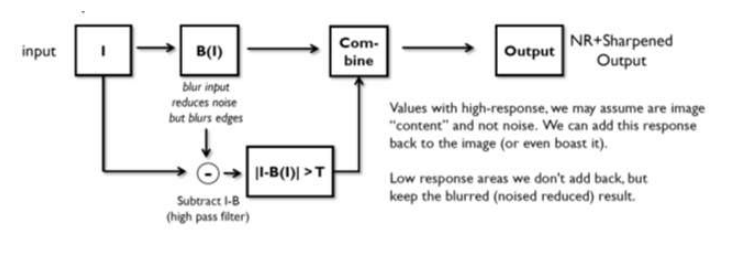
\includegraphics[width=0.5\textwidth]{img/denoising_gaussiano_adattivo.png}
    \caption{esempio di denoising adattivo sul gaussiano}
\end{figure}

\subsection{Automated correction}
La prima correzione automatica applicata è l'\textbf{autofocus} ed esistono diversi 
approcci:
\begin{itemize}
    \item \textbf{approcci attivi}: utilizzando gli infrarossi per calcolare la
    distanza del soggetto
    \item \textbf{passivi}: si analizza la frequenza spaziale dell'immagine per 
    stimare il focus come ad esempio il contrasto (più contrasto allora immagine a fuoco).
    Un esempio di autofocus è anche quello basato sugli edge e quindi usare il filtro 
    laplaciano.
    \item \textbf{smart}: si utilizzano i soggetti per mettere a fuoco, come le facce.
\end{itemize}

Abbiamo poi anche la selezione dell'\textbf{automated exposure}, ovvero la quantità 
di luce che entra e quindi il tempo di apertura dell'otturatore. In sostanza si 
effettua una media di intensità di alcuni pixel selezionati e utilizzare una soglia, esistono diverse maschere 
per selezionare i pixel. Possiamo anche basarci sulla skin-tone.

\begin{nota}
    PEr le camere HDR si effettuano multipli scatti e si effettua una combinazione
    delle immagini.
\end{nota}

Abbiamo anche l'\textbf{auto white balancing} si basa sulla stima del colore dell'illuminante 
della scena, per esempio sfruttando l'ipotesi di \textbf{grey world}. In sostanza 
si assume che un'immagine con una variazione di colori quando la continuiamo a sfocare 
arriveremo ad ottenere il colore grigio. Quando l'immagine non è bilanciata si ottiene 
il colore dell'illuminante e poi si applica la trasformazione. Il problema è che non 
otteniamo buoni risultati sempre.
\begin{nota}
    Prima avevamo visto il custom white balancing, ovvero quello supervisionato
    dove si utilizza una palette di reference o un oggetto bianco nella scena. La 
    versione automatica si basa sullo stimare l'illuminante e poi correggere.
\end{nota}

\end{document}